\documentclass[12pt]{article}

\usepackage{sbc-template}

\usepackage{graphicx,url}

\usepackage{listings}
\usepackage{xcolor}
\lstset { %
    language=C,
    %backgroundcolor=\color{black!5}, % set backgroundcolor
    basicstyle=\tiny,% basic font setting
}


\usepackage[brazil]{babel}   
%\usepackage[latin1]{inputenc}  
\usepackage[utf8]{inputenc}  
% UTF-8 encoding is recommended by ShareLaTex
\usepackage{multicol}
\usepackage[none]{hyphenat}
\newenvironment{Figure}
  {\par\medskip\noindent\minipage{\linewidth}}
  {\endminipage\par\medskip}     
\sloppy

\title{Relatório de Entrega - Exercício 3  \\
       Disciplina de programação Paralela (PP) Prof. César De Rose
       }

\author{Leonardo G. Carvalho(pp12816), Matheus S. Redecker(pp12819)}


%\address{Pontifícia Universidade Católica do Rio Grande do Sul - PUCRS
%  \email{  \{leonardo.gubert\}\{matheus.redecker\} @acad.pucrs.br}
%}


\begin{document} 


\maketitle

{\footnotesize
\begin{multicols}{2}
\section{Introdução}
O objetivo deste trabalho é implementar, utilizando as biblioteca de \textit{MPI} e \textit{OpenMP}, uma versão paralela de um programa que realiza a ordenação de linhas de uma matriz utilizando o modelo mestre e escravo. Os escravos devem seguir o modelo de \textit{workpool} em \textit{OpenMP}, disparando \textit{threads} para realizar a ordenação em paralelo. Os algoritmos de ordenação que serão testados são: \textit{Quick Sort} e \textit{Bubble Sort}.  A modelagem do problema foi feita pensando que os escravos precisam receber linhas da matriz, realizar a ordenação de cada linha por uma \textit{thread} diferente e, após finalizar, enviar de volta para o mestre as linhas ordenadas. Para isso ser realizado foi definido o ultimo processo como sendo o mestre, e os demais processos como escravos. 

\section{Implementação}
Como havia um problema para enviar e receber as linhas da matriz sem precisar enviar mais de uma mensagem, foi optado por utilizar uma simplificação proposta em aula. Cada linha da matriz conta como 8 linhas menores, por isso a quantidade de elementos presente em cada linha da matriz foi multiplicada pelo número de \textit{threads} desejada, e para compensar, o número total de linhas foi dividido pelo número de \textit{threads}, para que a quantidade de linhas se equivalha. \\
Quando o mestre é executado, a primeira coisa a ser feita é criar e alocar memória para a matriz principal, deviado ao fato de que nesse trabalho temos que executar o programa para dois algoritmos de ordenação diferentes, temos duas funções para alocação da matriz, para pegar o pior caso de ordenação de cada um dos vetores. Feito isso, o mestre realiza um \textit{burst} inicial, enviando para cada um dos escravos uma linha da matriz com uma \textit{tag} identificando qual a posição da linha que foi enviada. Após todos os escravos receberem uma linha, o mestre entra em um laço onde ele espera que qualquer escravo mande de volta a linha ordenada. Quando a mensagem é recebida, é feito um \textit{MPI\_Probe} para atualizar as informações de \textit{tag} e assim é feito um \textit{MPI\_Recv} endereçando o bloco recebido diretamente na linha correspondente através da informação da \textit{tag}. Se ainda existirem linhas a serem ordenadas, a próxima da sequencia é enviada para este escravo, senão, o mestre manda uma mensagem para finalizar o processo do escravo. Este laço do mestre é executado até que todas as linhas enviadas tenham sido recebidas ordenadas.\\
Para o escravo a tarefa é um pouco mais complexa. A primeira coisa a ser feita é alocar memoria para receber o vetor do mestre, após é preciso também alocar memoria para quando for necessário quebrar o vetor recebido em vetores menores de acordo com o número de \textit{threads} desejadas. Após isso o escravo entra em um laço onde é verificado se a \textit{tag} é para finalizar o processo. Se for, ele é finalizado, senão ele realiza a quebra do vetor em vetores menores. Uma vez tendo dividido os vetores, o escravo realiza a ordenação para cada um em um laço que pode ou não ser paralelizado utilizado o \textit{OpenMP} e quando a ordenação for finalizada o escravo une os vetores novamente para enviar para o mestre. 

\section{Dificuldades encontradas}
A principal dificuldade foi encontrar a maneira de enviar e receber uma maior quantidade de vetores, sem precisar enviar mais de uma mensagem. Esse problema foi solucionado aumentando o tamanho de elementos dentro de cada linha, de acordo com o número de \textit{threads} desejada que seja ordenado dentro de cada nodo. Assim quando o escravo tiver que ordenar, ele irá dividir a linha recebida pelo número de \textit{threads} representando quantos vetores serão ordenados.

\section{Testes}
Os testes foram executados com a alocação de 4 nodos no \textit{cluster} Atlantica. Foi utilizado 5 processos, sendo 1 mestre e 4 escravos. O mestre está situado no ultimo processo, e no mesmo nodo irá ter um processo escravo. A ordenação foi feita com 10.000 vetores de 100.000 elementos para o algoritmo de \textit{Quick Sort} e 10.000 vetores de 10.000 elementos para o algoritmo de \textit{Bubble Sort}, os vetores foram gerados como o pior caso de ordenação para cada algoritmo especifico. O número de \textit{threads} em cada nodo foi variado entre 1, 8 e 16. A comparação foi feita entre a versão paralela com as \textit{threads} e a outra sem \textit{OpenMP}, com isso deixando os processos escravos mais pesados, pois devem ordenar os vetores de forma sequencial.

\section{Análise de desempenho}

A versão utilizando \textit{OpenMP} com as \textit{threads} em paralelo obteve um desempenho superior a versão dos escravos com carga pesada. A partir do comportamento do desempenho podemos concluir que o \textit{Bubble Sort} se beneficiou mais do paralelismo pois o salto de \textit{speedup} é consideravelmente maior. Isso ocorre porque esse algoritmo tem uma complexidade quadrática, e quando paralelizado o ganho é maior do que no algoritmo do \textit{Quick Sort}, pois ele é tão rápido que realiza a ordenação dos vetores rapidamente, e por essa razão a diferença entre as versões, com e sem \textit{OpenMP} não é tão expressiva. A utilização de \textit{hyper-threading} não obteve um ganho maior em nenhum dos casos, mas manteve o mesmo índice, perdendo um pouco sua eficiência pelo fato de que está utilizando mais \textit{threads} para não obter ganho no tempo.

\begin{Figure}
\centering
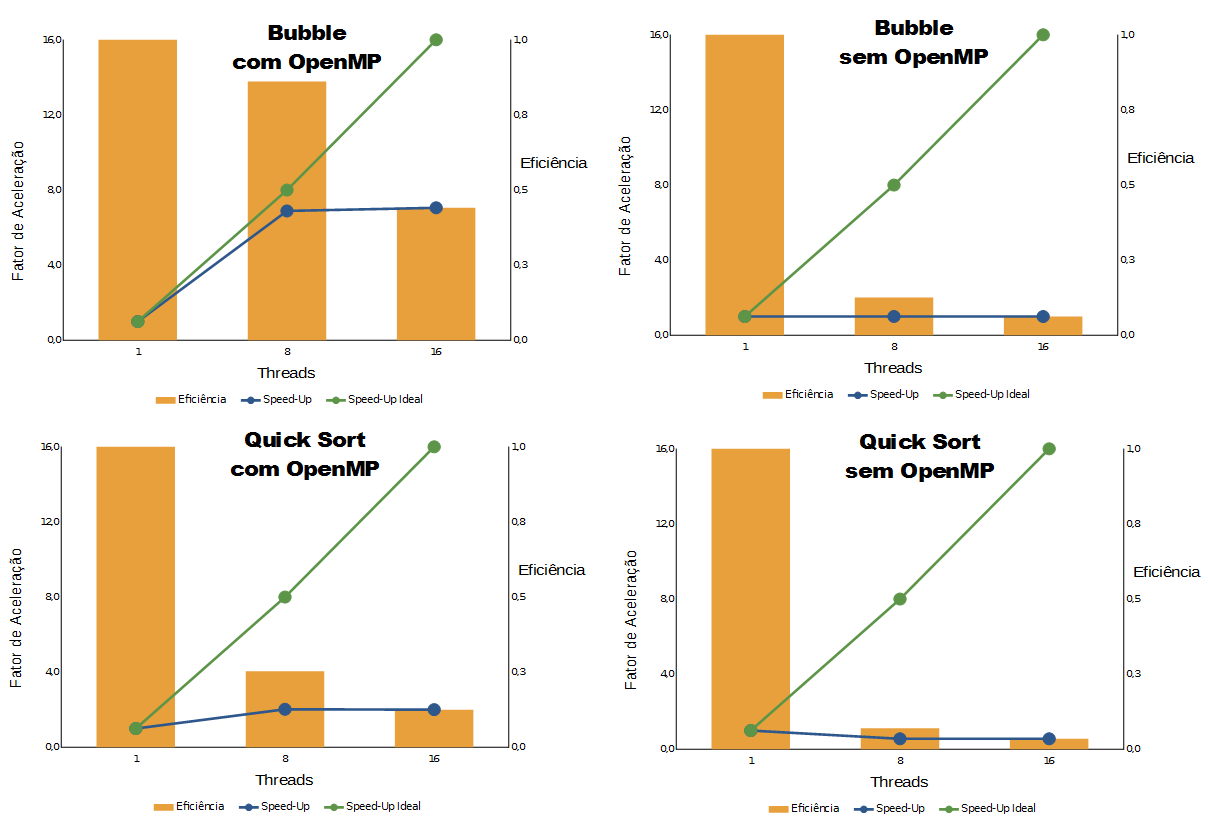
\includegraphics[width=\columnwidth]{fig/new.png}
\label{fig:grafico}
\end{Figure}


\section{Observações finais} 
É possível concluir que este problema possui um melhor desempenho quando utilizado o paralelismo através do \textit{OpenMP}, onde o ganho é obtido na ordenação dos vetores de forma paralela. Isso é possível pois os vetores não tem ligação entre si. Quando cada \textit{thread} ordena um vetor separado o tempo diminui, quando comparado com a versão sequencial. 

\end{multicols}

\newpage{}
\section{Código}

}

\begin{lstlisting}
#include <stdio.h>
#include <stdlib.h>
#include "mpi.h"
#include <omp.h>
#include <string.h>


#define PACK_SIZE 8 //Numero de linhas que sao enviados no pacote
#define MATRIX_LINES 10000 / PACK_SIZE //numero de linhas na matriz
#define MATRIX_COLUMNS 10000 * PACK_SIZE //numero de elementos em cada linha da matriz
#define THREAD_COLUMNS MATRIX_COLUMNS / PACK_SIZE //Numero de elementos que cada vetor contem dentro da linha
#define SUICIDE_TAG 666666

int *theMatrix[MATRIX_LINES];
int *slaveBuffer;

void createMatrixQuick()
{
   //Aloca a matriz
    int i, j;
    for (i = 0; i < MATRIX_LINES; i++){
        theMatrix[i] = malloc(sizeof(int) * MATRIX_COLUMNS);
    }
   //Preenche
    for (i = 0; i < MATRIX_LINES; i++){
        for(j = 0; j<MATRIX_COLUMNS; j++){
            theMatrix[i][j] = MATRIX_COLUMNS - j + (10*i);
        }
    }
}

void createMatrixBubble()
{
   //Aloca a matriz
    int i, j;
    for (i = 0; i < MATRIX_LINES; i++){
        theMatrix[i] = malloc(sizeof(int) * MATRIX_COLUMNS);
    }
   //Preenche
    for (i = 0; i < MATRIX_LINES; i++){
        for(j = 0; j<MATRIX_COLUMNS; j++){
            theMatrix[i][j] = MATRIX_COLUMNS - j;
        }
    }
}

int cmpfunc (const void * a, const void * b)
{
   return ( *(int*)a - *(int*)b );
}

void bs(int n, int * vetor){
	int c=0, d, troca, trocou =1;
	while (c < (n-1) & trocou ){
		trocou = 0;
		for (d = 0 ; d < n - c - 1; d++)
			if (vetor[d] > vetor[d+1]) {
				troca      = vetor[d];
				vetor[d]   = vetor[d+1];
				vetor[d+1] = troca;
				trocou = 1;
				}
		c++;
		}
}

int main(int argc, char** argv)
{
    int my_rank;  // Identificador do processo
    int proc_n;   // Numero de processos
    int nextVector; //Qual a posicao do proximo vetor a ser enviado
    int receivedVectors = 0; // Quantos vetores ja foram recebidos 
    MPI_Status status; // Status de retorno

    MPI_Init (&argc, &argv);

    MPI_Comm_rank(MPI_COMM_WORLD, &my_rank);
    MPI_Comm_size(MPI_COMM_WORLD, &proc_n);
    
    //MESTRE
    if (my_rank == proc_n-1){
	    //utilizado para contagem do tempo
	    double t1,t2;
	    t1 = MPI_Wtime();
 
        //Cria a matriz original
        createMatrixQuick();
        //createMatrixBubble();

        //Faz a distribuicao inicial
        for(nextVector = 0; nextVector < proc_n-1; nextVector++){
            MPI_Send(theMatrix[nextVector], MATRIX_COLUMNS,
            MPI_INT, nextVector, nextVector, MPI_COMM_WORLD);
        }

        // Enquanto ainda ha linhas a serem ordenadas
        while(receivedVectors<MATRIX_LINES){
            //Recebe a linha ordenada
            //e envia outra para o mesmo escravo
            MPI_Probe(MPI_ANY_SOURCE, MPI_ANY_TAG, 
                      MPI_COMM_WORLD, &status);
            MPI_Recv (theMatrix[status.MPI_TAG], MATRIX_COLUMNS,
                      MPI_INT, MPI_ANY_SOURCE, MPI_ANY_TAG,
                      MPI_COMM_WORLD, &status);
            receivedVectors++;

            //Se ainda ha vetores a serem enviados, manda ele.
            if(nextVector<MATRIX_LINES) {
                MPI_Send (theMatrix[nextVector], MATRIX_COLUMNS,
                          MPI_INT, status.MPI_SOURCE,
                          nextVector, MPI_COMM_WORLD);
                nextVector++;
            }
        
            //se nao manda o processo finalizar
            else{
                int nada = 10;
                MPI_Send (&nada, 1, MPI_INT, status.MPI_SOURCE,
                          SUICIDE_TAG, MPI_COMM_WORLD);
            }
        }
	    t2 = MPI_Wtime(); // termina a contagem do tempo
	    printf("\nTempo de execucao: %f\n\n", t2-t1);
    }
    //ESCRAVOS
    else {

        //Inicializa o buffer de recebimento
        slaveBuffer = malloc(sizeof(int) * MATRIX_COLUMNS);

        //inicializa o buffer de matrizes
        int *slaveMatrix[PACK_SIZE];
        int i;
        for (i = 0; i < PACK_SIZE; i++){
            slaveMatrix[i] = malloc(sizeof(int) * THREAD_COLUMNS);
        }

        while(1){
            //Recebe as linhas para ordenar
            MPI_Recv (slaveBuffer, MATRIX_COLUMNS, MPI_INT, 
                      proc_n-1, MPI_ANY_TAG, MPI_COMM_WORLD,
                      &status);
            if(status.MPI_TAG == SUICIDE_TAG){
                break;
            }

            //Faz a divisao do vetor em PACK_SIZE vetores
            int linha = -1;
            int coluna = 0;
            for(i = 0; i < MATRIX_COLUMNS; i++){
                if(i % THREAD_COLUMNS == 0){
                    linha++;
                    coluna=0;  
                } 
                slaveMatrix[linha][coluna] = slaveBuffer[i];
                coluna++;
            }

            //Faz a ordenacao nos vetores
            #pragma omp parallel for
            for(i = 0; i < PACK_SIZE; i++){
                qsort(slaveMatrix[i], THREAD_COLUMNS, sizeof(int), cmpfunc);
            	//bs(THREAD_COLUMNS, slaveMatrix[i]);
	    	}

            //Junta tudo no buffer novamente            
            int elemento = 0;
            int j;
            for(i = 0; i < PACK_SIZE; i++){
                for(j = 0; j < THREAD_COLUMNS; j++){
                    slaveBuffer[elemento] = slaveMatrix[i][j];
                    elemento++;
                }
            }

            //retorna para o mestre
            MPI_Send (slaveBuffer, MATRIX_COLUMNS, MPI_INT,
                      proc_n-1, status.MPI_TAG, MPI_COMM_WORLD);
        }
    }
    MPI_Finalize();
}
\end{lstlisting}

\end{document}



